\documentclass[conference]{IEEEtran}
\IEEEoverridecommandlockouts
\usepackage{biblatex}
\usepackage{amsmath,amssymb,amsfonts}
\usepackage{algorithmic}
\usepackage{graphicx}
\usepackage{textcomp}
\usepackage{xcolor}
\usepackage{enumitem}

\addbibresource{Bacherlor_Seminar.bib}

\begin{document}

\title{Haptisches Feedback eines Roboters durch virtuelle 3D-Modelle}

\author{
    \IEEEauthorblockN{Carl Gathmann}
    \IEEEauthorblockA{\textit{Universität zu Lübeck}\\
        Lübeck, Germany \\
        carl.gathmann@student.uni-luebeck.de}
    \and
    \IEEEauthorblockN{Marten Buchmann}
    \IEEEauthorblockA{\textit{Universität zu Lübeck}\\
        Lübeck, Germany \\
        marten.buchmann@student.uni-luebeck.de}
}
\maketitle

\begin{abstract}
!!!NOCH GPT!!!
In dieser Studie wird ein Ansatz zur Generierung von haptischem Feedback in Mensch-Roboter-Interaktionen vorgestellt. Mittels maßgeschneiderter Software erzeugen wir eine sensorische Wahrnehmung, die durch frei gestaltbare, virtuelle 3D-Modelle gesteuert wird. Der Anwender erfährt eine Art abweisende Kraft, die durch die räumlichen Grenzen des virtuellen Modells definiert ist, wodurch eine physische Interaktion mit dem immateriellen Modell simuliert wird. Die vorgestellte Technologie findet breite Anwendungsbereiche, von medizinischen Simulationen und Exploration in gefährlichen Zonen bis hin zur Erhöhung der Spielerfahrung in virtuellen Umgebungen. In Verbindung mit Virtual-Reality-Ausrüstung eröffnet unsere Methode neue Wege zur Verbesserung der Benutzerimmersion durch die Vermittlung eines realistischeren Gefühls für die Form und Textur virtueller Objekte. Die in dieser Arbeit vorgestellten Prinzipien und Implementierungen können als Grundlage für weiterführende Forschungen und Entwicklungen auf diesem aufstrebenden Gebiet dienen.
\end{abstract}

\begin{IEEEkeywords}
    component, formatting, style, styling, insert
\end{IEEEkeywords}

\section{Introduction}
!!! GPT =>

Die Mensch-Roboter-Interaktion hat in den letzten Jahren zunehmend an Bedeutung gewonnen und sich als ein dynamisches Forschungs- und Anwendungsfeld etabliert. Im Zentrum dieser Interaktion steht die Verbesserung der Benutzererfahrung durch die Erweiterung der sinnlichen Wahrnehmung des Menschen.

In dieser Studie präsentieren wir einen Ansatz, der es dem Benutzer ermöglicht, virtuelle 3D-Modelle zu "ertasten", indem er über ein Roboterinterface mit ihnen interagiert. Dies wird durch die Erzeugung einer abweisenden Kraft erreicht, die auf den Grenzen der virtuellen Modelle basiert. Dieses haptische Feedback simuliert das physische Berühren eines realen Objekts, obwohl kein tatsächlicher physischer Kontakt mit dem virtuellen Modell besteht. 

Dieser Ansatz bietet zahlreiche Anwendungsmöglichkeiten, darunter die Simulation von Operationen für Ausbildungszwecke, die Erkundung von Objekten in gefährlichen oder unzugänglichen Umgebungen und die Erhöhung der Immersion in virtuellen Spielen. Darüber hinaus kann die Kombination unserer Technologie mit Virtual-Reality-Brillen zu einem verbesserten Gefühl von Präsenz und Realismus in virtuellen Umgebungen führen.

Das vorliegende Paper beleuchtet die zugrundeliegenden Prinzipien, technische Details und potenzielle Anwendungen dieses Ansatzes. Es leistet einen wertvollen Beitrag zur Erforschung und Weiterentwicklung von Technologien für haptisches Feedback in der Mensch-Roboter-Interaktion.

<= GPT !!!

\section{Methods}

Während der Recherche des Projekts wurden verschiedene Ansätze zur Erzeugung von haptischem Feedback in der Mensch-Roboter-Interaktion untersucht, welche in den folgenden Abschnitten vorgestellt werden.

Als Vorbereitung  auf die Verwendung der Ansätze muss zuerst ein zweidimensionales Problem aus dem dreidimensionalen Problem gemacht werden. Erreicht wird dies durch die Erstellung eines neuen Koordinatensystems für jedes Dreieck, welches sich ergibt durch:
\begin{enumerate}
    \item Eine Kante des Dreiecks als x-Achse
    \item Das Kreuzprodukt der entstandenen Achse mit einem weiteren Vektor als z-Achse
    \item Das Kreuzprodukt der beiden entstandenen Achsen als y-Achse
\end{enumerate}
Die Koordinaten des Punktes werden dann in diesem Koordinatensystem angegeben. Auf diese Art repräsentieren die x- und y-Koordinaten die Position und die z-Koordinate die Entfernung des Punktes von der Ebene des Dreiecks. 

\subsection{Edge Funktion}
Die Edge-Funktion ist eine häufig verwendete Funktion im Bereich der Computer-Grafik. Sie wird verwendet, um herauszufinden, wo sich ein Punkt relativ zu einem Dreieck befindet. Definiert ist sie wie folgt:
\begin{equation}
    E_{i} = (x_{i+1} - x_{i})(y - y_{i}) - (y_{i+1} - y_{i})(x - x_{i})
\end{equation}
x, y sind die Koordinaten des Punktes, $x_{i}$, $y_{i}$ sind die Koordinaten des i-ten Eckpunktes des Dreiecks.
Im Fall eines Dreiecks mit den Eckpunkten $A$, $B$ und $C$ und einem Punkt $P$ ist der Punkt innerhalb des Dreiecks, wenn gilt:
\begin{equation}
    E_{AB} \geq 0 \land E_{BC} \geq 0 \land E_{CA} \geq 0
\end{equation}

!!!BILD!!!

Mit dem Wissen, ob ein Punkt innerhalb des Dreiecks liegt und der Höhe des Punktes, die über die z-Koordinate des transformierten Punktes gegeben ist, kann ein Kraftvektor berechnet werden. Dieser Kraftvektor zeigt in Richtung der Normalen des Dreiecks und ist proportional zur Höhe des Punktes. Die Kraft kann dann wie folgt berechnet werden:
\begin{equation}
    F = \frac{1}{d} \cdot n
\end{equation}
$d$ ist die Entfernung des Punktes von der Ebene des Dreiecks und $n$ ist die Normale des Dreiecks.
Die großen Vorteile dieser Methode sind die Einfachheit und die Geschwindigkeit. Die Berechnung der Edge-Funktion ist sehr einfach und schnell, da sie nur 2 Multiplikationen und 4 Subtraktionen benötigt.
Ein Problem, was sich daraus ergibt, ist die Unstetigkeit entlang der Kanten benachbarter Dreiecke. Dies kann zu unintuitivem und sprunghaftem Verhalten führen, wenn der Benutzer sich entlang der Kante bewegt. Aus diesem Grund haben wir die Methode verworfen und uns an einer weiteren Methode versucht.

\subsection{Baryzentrische Koordinaten}
Eine weitere Methode, die wir untersucht haben, ist die Verwendung von baryzentrischen Koordinaten. Diese Methode ist sehr ähnlich zur Edge-Funktion, da sie auch verwendet wird, um herauszufinden, wo sich ein Punkt relativ zu einem Dreieck befindet. Definiert ist sie wie folgt:
\begin{equation*}
    \lambda_1 = \frac{(y_{B} - y_{C})(x_{P} - x_{C}) + (x_{C} - x_{B})(y_{P} - y_{C})}{(y_{B} - y_{C})(x_{A} - x_{C}) + (x_{C} - x_{B})(y_{A} - y_{C})}
\end{equation*}
\begin{equation}
    \lambda_2 = \frac{(y_{C} - y_{A})(x_{P} - x_{C}) + (x_{A} - x_{C})(y_{P} - y_{C})}{(y_{B} - y_{C})(x_{A} - x_{C}) + (x_{C} - x_{B})(y_{A} - y_{C})}
\end{equation}
\begin{equation*}
    \lambda_3 = 1 - \lambda_1 - \lambda_2
\end{equation*}
A, B, C sind hierbei die Eckpunkte des Dreiecks und P die in das Koordinatensystem des Dreiecks transformierte Roboter Position. $\lambda_1$, $\lambda_2$ und $\lambda_3$ sind die baryzentrischen Koordinaten des Punktes P. Diese sagen aus wie weit der Punkt von den jeweiligen Eckpunkten entfernt ist. Wenn alle drei Koordinaten positiv sind, liegt der Punkt innerhalb des Dreiecks. Nun lässt sich ein Schwellwert festlegen, ab dem eine Interpolation zwischen den Kanten/Eckpunkten des Dreiecks stattfindet. Dazu ist es notwendig, für jede Kante zu wissen, welche Dreiecke sie enthält und welche Normalen diese Dreiecke haben. Das gleiche gilt für die Eckpunkte. Anschließend kann die Kraft wie folgt berechnet werden:
\begin{equation*}
    F_{ab} = 
    \begin{cases} 
        \lambda_1 \frac{{ F_{AB1} + F_{AB2} + \ldots + F_{ABn}}}{n} &  0 < \lambda_1 < \text{Schwellwert}, \\
        0 & \text{sonst.}
    \end{cases}
\end{equation*}
\begin{equation*}
    F_{bc} =
    \begin{cases} 
        \lambda_2 \frac{{ F_{AB1} + F_{AB2} + \ldots + F_{ABn}}}{n} &  0 < \lambda_2 < \text{Schwellwert}, \\
        0 & \text{sonst.}
    \end{cases}
\end{equation*}
\begin{equation*}
    F_{ca} =
    \begin{cases} 
        \lambda_3 \frac{{ F_{AB1} + F_{AB2} + \ldots + F_{ABn}}}{n} &  0 < \lambda_3 < \text{Schwellwert}, \\
        0 & \text{sonst.}
    \end{cases}
\end{equation*}
$F_1, F_2, \ldots, F_n$ sind die Normalen der Dreiecke, die die jeweilige Kante enthalten. $F_{ab}$ ist die Kraft, die auf den Benutzer wirkt, wenn er sich auf der Kante zwischen den Punkten A und B befindet. $F_{bc}$ und $F_{ca}$ sind analog dazu.

Für die Eckpunkte gilt der gleiche Ansatz nur sind hier zwei Bayzentrische Koordinaten gleichzeitig zwischen 0 und Schwellwert. Entsprechend wird die Kraft wie folgt berechnet:
\begin{equation*}
    F_{a} = 
    \begin{cases} 
        \frac{(\lambda_1 + \lambda_2)}{2} \frac{{ F_{A1} + F_{A2} + \ldots + F_{An}}}{n} &  0 < \lambda_1, \lambda_2 < \text{Schwellwert} \\
        0 & \text{sonst.}
    \end{cases}
\end{equation*} 
\begin{equation*}
    F_{b} = 
    \begin{cases} 
        \frac{(\lambda_2 + \lambda_3)}{2} \frac{{ F_{A1} + F_{A2} + \ldots + F_{An}}}{n} &  0 < \lambda_2, \lambda_3 < \text{Schwellwert} \\
        0 & \text{sonst.}
    \end{cases}
\end{equation*} 
\begin{equation*}
    F_{c} = 
    \begin{cases} 
        \frac{(\lambda_3 + \lambda_1)}{2} \frac{{ F_{A1} + F_{A2} + \ldots + F_{An}}}{n} &  0 < \lambda_3, \lambda_1 < \text{Schwellwert} \\
        0 & \text{sonst.}
    \end{cases}
\end{equation*} 
Der Vorteil gegenüber der Edge-Funktion ist, dass so die Unstetigkeit entlang der Kanten vermieden wird, die Berechnung der baryzentrischen Koordinaten ist jedoch etwas komplexer und langsamer als die Berechnung der Edge-Funktion. Daher wurde auch diese Variante letztendlich nicht verwendet.

\subsection{Point-Triangle-Distance-Funktion}
















Die Erzeugung des haptischen Feedbacks beruht auf der Berechnung einer abweisenden Kraft, die so konzipiert ist, dass sie dem Benutzer ein realistisches Gefühl für die Form des virtuellen 3D-Modells vermittelt. Der Kern dieser Technik basiert auf der Nutzung des weit verbreiteten und flexiblen STL-Standards, der allgemein in der Industrie zur Speicherung und Übertragung von 3D-Modellen eingesetzt wird.

Für die physische Implementierung der Mensch-Roboter-Interaktion wurde der Panda-Roboter von Franka Emika ausgewählt. Der Panda zeichnet sich durch seine 7-achsige Struktur aus, die hohe Präzision und Flexibilität bietet. Eine benutzerfreundliche, 3D-gedruckte Schnittstelle (\ref{fig:nullSpace}) wurde am Endeffektor des Roboters installiert, um die Führung durch menschliche Benutzer zu erleichtern.  

\begin{figure}
    \centering
    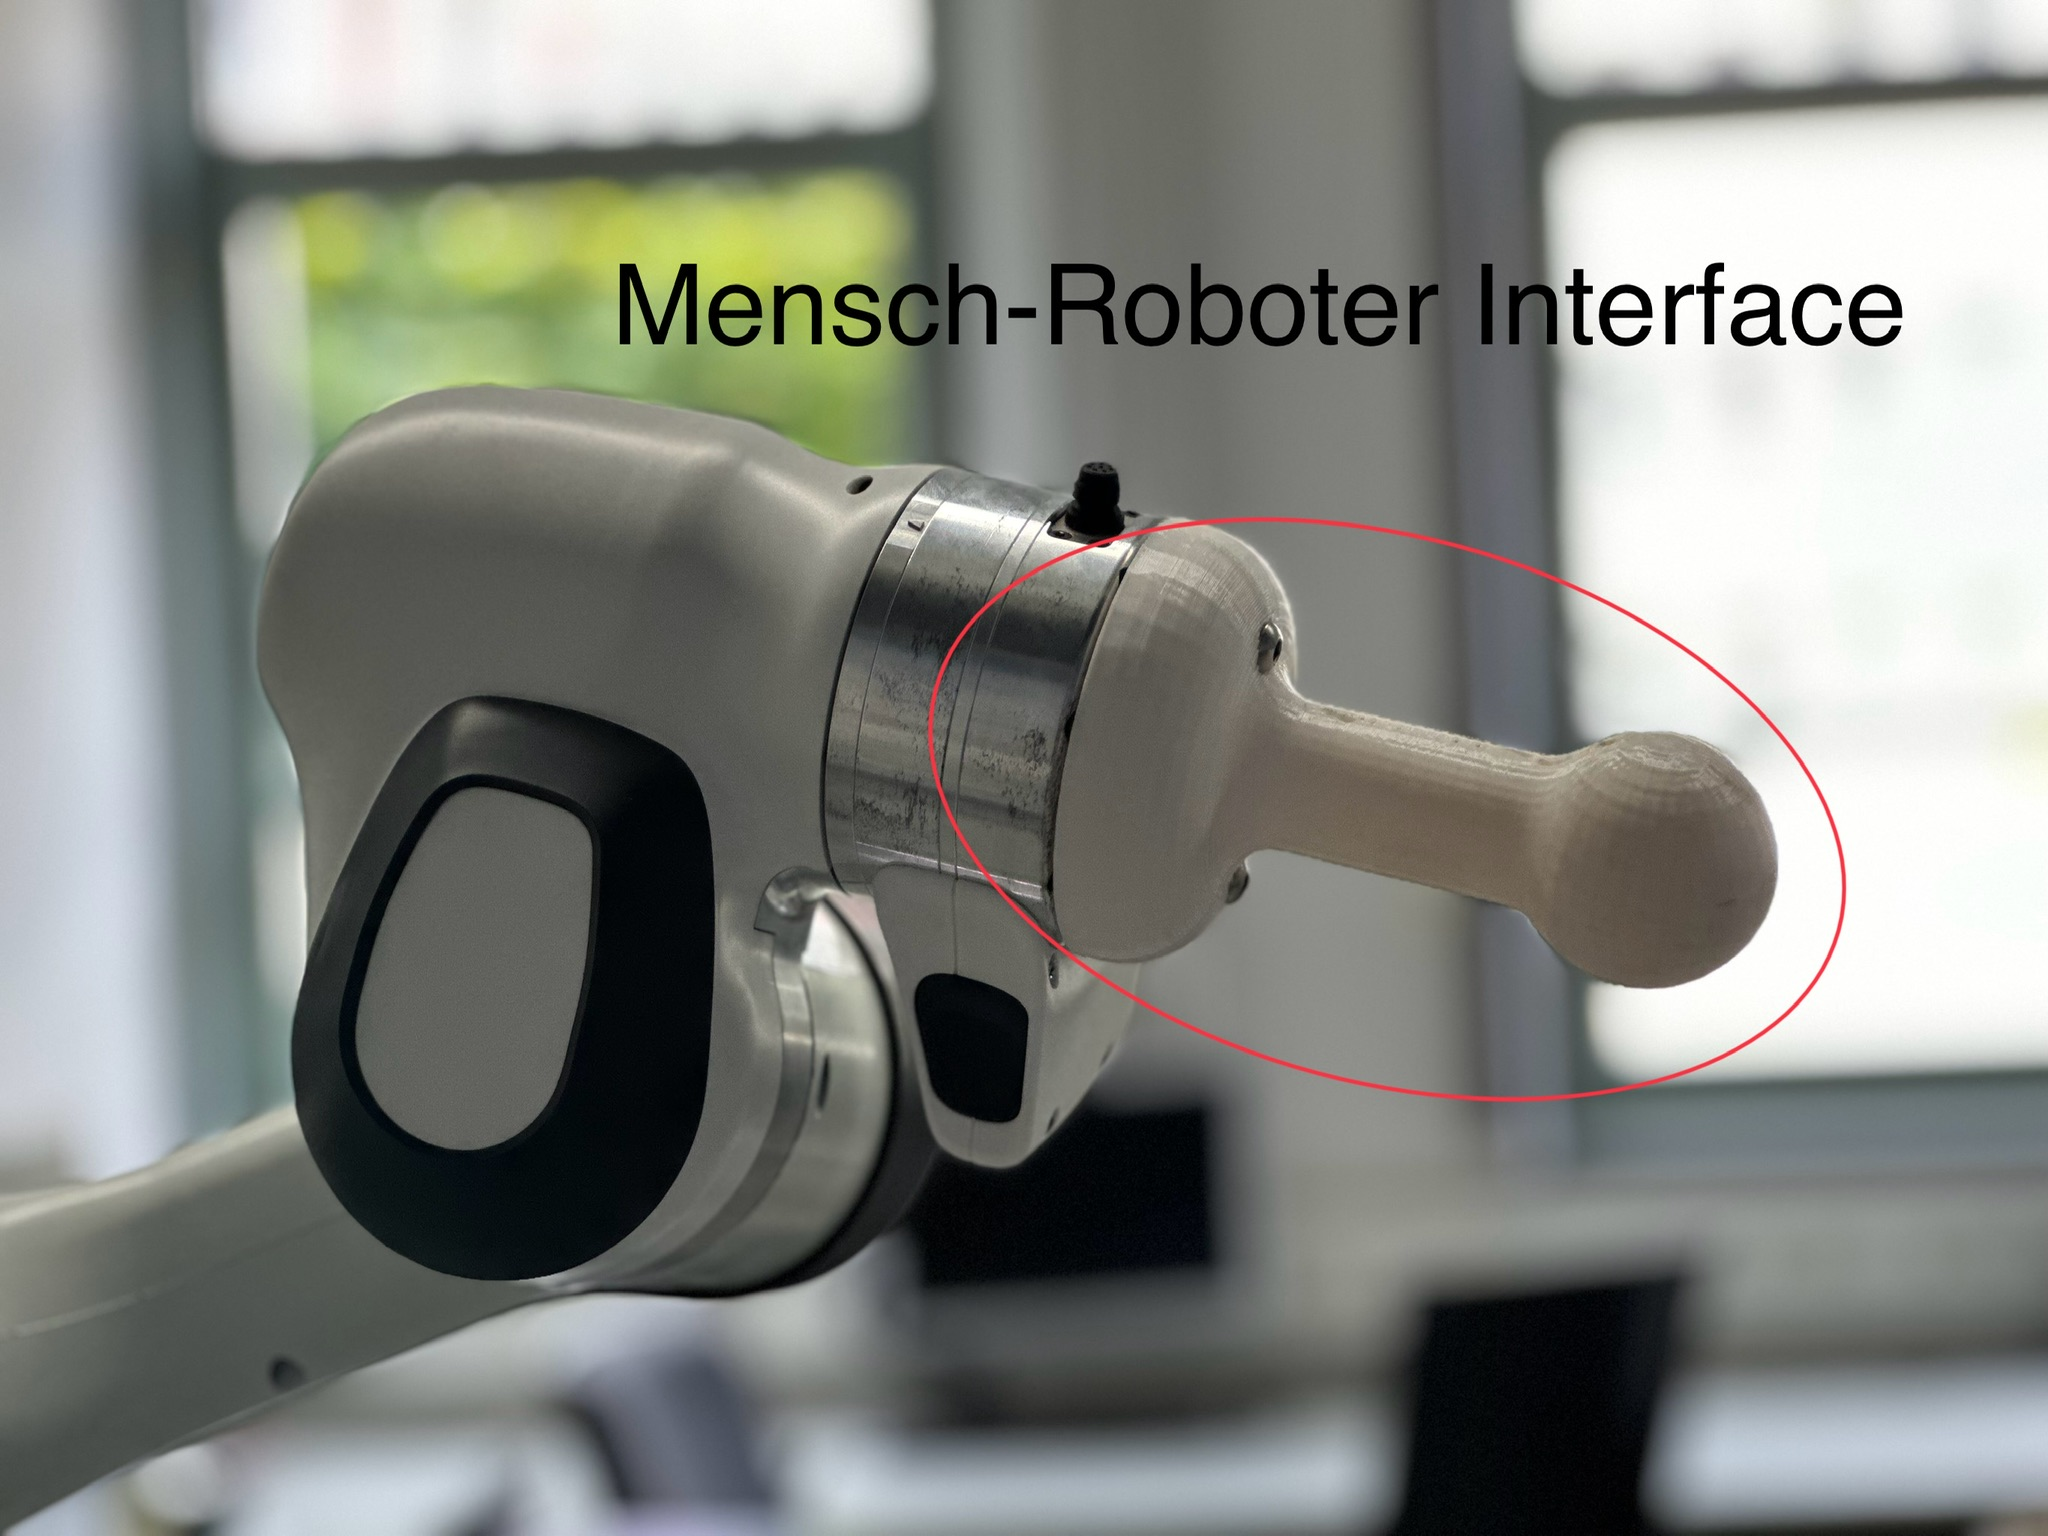
\includegraphics[width=0.45\textwidth]{pics/interface.jpeg}
    \caption{Mensch-Roboter-Schnittstelle}
    \label{fig:nullSpace}
\end{figure}

Bei der Entwicklung der Software für dieses System stand die Leistungsfähigkeit im Vordergrund, um eine nahtlose Benutzererfahrung zu gewährleisten. Dazu war es entscheidend, dass die Anwendung in Echtzeit ausgeführt werden kann, wobei eine maximale Zeitverzögerung von weniger als 1 Millisekunde akzeptiert wurde. Die Programmiersprache C++ wurde aufgrund ihrer hohen Performance ausgewählt, um diesem Anspruch gerecht zu werden. Die Hardware-Konfiguration bestand aus [!!!HARDWARE!!!].

Die Verarbeitung und Nutzung der 3D-Modelle wurden durch die Umwandlung der STL-Daten in Eigen-Matrizen optimiert. Dieser Prozess wurde durch einen STL-Parser ermöglicht und ermöglichte eine einfache und effiziente Handhabung der 3D-Daten innerhalb des Systems.

Insgesamt zeichnet sich unsere Methodik durch die Kombination von Standardtechnologien und innovativen Ansätzen aus, um eine effiziente und benutzerfreundliche Lösung für haptisches Feedback in der Mensch-Roboter-Interaktion zu schaffen.

\section{Results}

\section{Discussion}

\section{Conclusion}

\printbibliography

\end{document}